% !TEX root = main.tex
% en preliminär beskrivning av angreppssätt
\chapter{Method}\label{cha:method}
This thesis will identify possible control approaches that could be applicable to the rotational stage at \abbrCERN in order to meet the performance requirements. The work is divded into three major subblocks; Identification of control approaches, Simulations and Implementation on real device.


\section{Identification of control approaches}
First of all, a brief analysis of the already developed controller will be done in order to point out the drawbacks and determine which controller qualities that have to be improved in order to achieved the desired performance during linear movement of the system. Moreover will a comprehensive literture study be done to understand the dynamics and identify possible control approaches. The main work will then consist of investigating different control approaches such as feedforward, H-infinity, iterative or state feedback control.

\section{Simulations}
After identifying a handful control approaches that could be applicable to this problem, simulations and implementaion will be done in Matlab and Simulink. The most promising approaches will be benchmarked in simulations and compared to the existing algorithm.

\section{Implementation on real device}
Finally, the most promising alternative will be implemented and tested on the real rotational stage. This will be done by implementating the control agorithm in Labview. The algorithm will run on a National Instruments PXI which will send the control signal and read the sensordata from the interferometer system.

\section{Timeplan}
%en tidplan för examensarbetets genomförande inklusive planerade datum för halvtidskontroll och framläggning
Figure~\ref{fig:timeplan} shows the timeplan for the master thesis project. \emph{HP} and \emph{FP} stands for halftime presentation and fulltime presentation, respectively. In addition to the master thesis work, some hardware testing will be carried out from time to time, throughout the whole thesis period.

\begin{figure}[h] %tbp
 \centering %crop: left bottom right top
 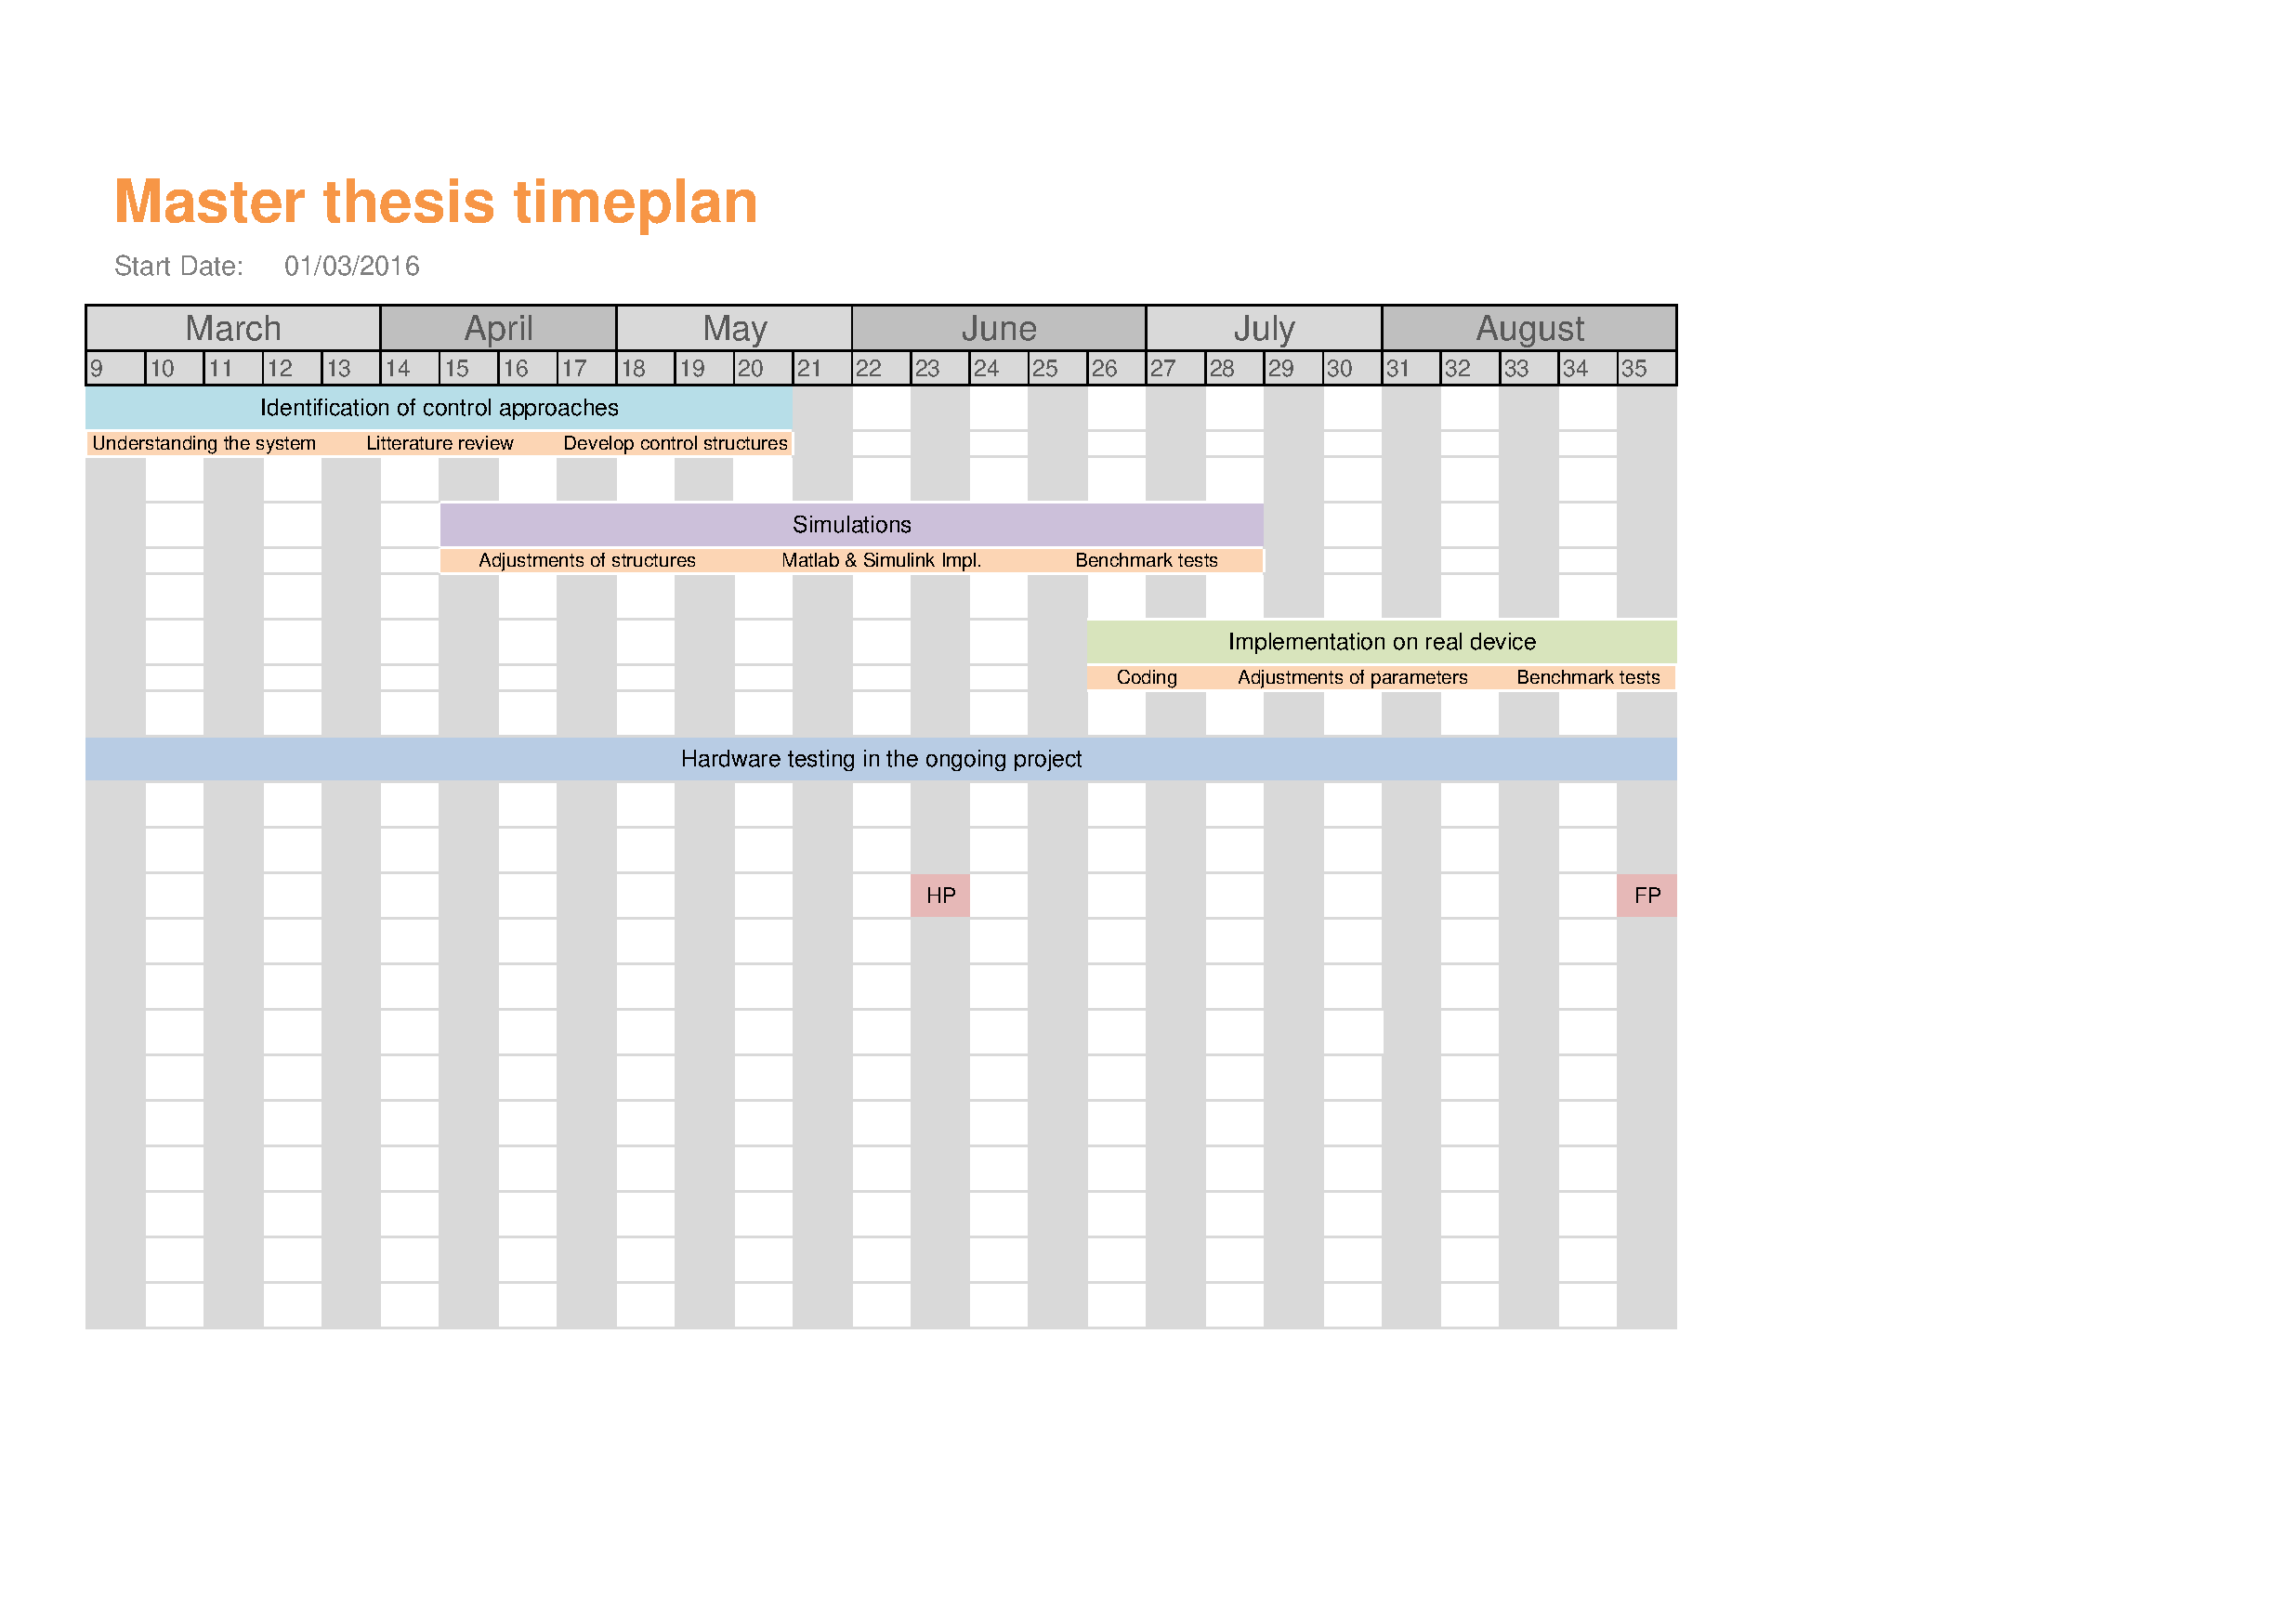
\includegraphics[trim=1cm 12cm 5cm 5.5cm, clip=true, scale=0.42]{fig/timeplan}
 \caption{\label{fig:timeplan}%
 Master Thesis timeplan, HP = Halftime presentation, FP = Fulltime presentation}
 \end{figure}
